\documentclass[10pt]{beamer}

\usetheme{metropolis}
% \metroset{sectionpage=simple}
\metroset{numbering=fraction}
\metroset{block=fill}
\definecolor{mLightBlue}{HTML}{0DA7FF}
\definecolor{TolLightRed}{HTML}{CC6677}

\usepackage{headings/kmath}
% Tikz
\usetikzlibrary{calc}
\usetikzlibrary{mindmap,trees,shapes,arrows,backgrounds,topaths}
\usetikzlibrary{decorations.pathmorphing, shapes.geometric}

% Text
\usepackage{enumitem}
\usepackage{ulem}
\usepackage{pifont}

% Maths
\usepackage{amsmath}
\usepackage{amsfonts}
\usepackage{amsthm}
\usepackage{amsopn}

% Plots
\usepackage{pgfplots}
\usepgfplotslibrary{groupplots}

% Tables
\usepackage{booktabs}
\usepackage{array}
\newcolumntype{L}{>$l<$}
\arraycolsep=1.4pt
\setlength{\tabcolsep}{3pt}

% Algos
\usepackage[ruled]{algorithm2e}

% Pgfplot
\pgfplotsset{
    legend image code/.code={
        \draw[mark repeat=2,mark phase=2] plot coordinates {
            (0cm,0cm)
            (0.25cm,0cm)
            (0.25cm,0cm)
        };
    }
}
% Objective values and functions
\newcommand{\pobj}{p}
\newcommand{\robj}{r}
\newcommand{\dobj}{d}

% Variables
\newcommand{\pvletter}{x}
\newcommand{\dvletter}{u}
\newcommand{\bvletter}{z}
\newcommand{\pv}{\mathbf{\pvletter}}
\newcommand{\dv}{\mathbf{\dvletter}}
\newcommand{\bv}{\mathbf{\bvletter}}
\newcommand{\pvi}[1]{\pvletter_{#1}}
\newcommand{\dvi}[1]{\dvletter_{#1}}
\newcommand{\bvi}[1]{\bvletter_{#1}}

% Problem data
\newcommand{\pdim}{n}
\newcommand{\ddim}{m}
\newcommand{\dic}{\mathbf{A}}
\newcommand{\obs}{\mathbf{y}}
\newcommand{\reg}{\lambda}
\newcommand{\regtwo}{\gamma}
\newcommand{\lfunc}{f}
\newcommand{\pfunc}{h}
\newcommand{\rfunc}{g}
\newcommand{\mcpone}{\boldsymbol{\alpha}}
\newcommand{\mcptwo}{\boldsymbol{\beta}}
\newcommand{\bigM}{M}


% Indices
\newcommand{\idxentry}{i}

% BnB
\newcommand{\pset}{\mathcal{X}}
\newcommand{\setidx}{\mathcal{S}}
\newcommand{\setzero}{\setidx_0}
\newcommand{\setone}{\setidx_1}
\newcommand{\setnone}{\setidx_\bullet}
\newcommand{\nodeSymb}{\nu}
\newcommand{\node}[1]{#1^{\nodeSymb}}
\newcommand{\pertslope}{\tau}
\newcommand{\pertlimit}{\mu}

% Math operators
\DeclareMathOperator{\diag}{diag}
\DeclareMathOperator{\dom}{dom}
\DeclareMathOperator{\interior}{int}

% Math misc
\newcommand{\1}{\mathbf{1}}
\newcommand{\0}{\mathbf{0}}
\newcommand{\abs}[1]{|#1|}
\newcommand{\biconj}[1]{#1^{**}}
\newcommand{\conj}[1]{#1^{*}}
\newcommand{\Id}{\mathbf{I}}
\newcommand{\icvx}{\mathbf{I}}
\newcommand{\intervint}[2]{[#1,#2]}
\newcommand{\iter}[2]{#1^{(#2)}}
\newcommand{\norm}[2]{\|#1\|_#2}
\newcommand{\opt}[1]{#1^{\star}}
\newcommand{\separable}[2]{#1_{#2}}
\newcommand{\subdiff}{\partial}
\newcommand{\transp}[1]{#1^{\mathrm{T}}}

% Abbreviations
\newcommand{\ie}{\textit{i.e.}}
\newcommand{\eg}{\textit{e.g.}}
\newcommand{\etal}{\textit{et al.}}


\setlength\fboxsep{5pt}
\setlength\fboxrule{1.5pt}


\begin{document}

\begin{frame}[plain,noframenumbering]
  \begin{center}
    {\large\textbf{Towards Stronger Relaxations for \\ $\boldsymbol{\ell}_{\boldsymbol{0}}$-Regularized Problems}}
  \end{center}
  \begin{center}
    Théo Guyard \\
    Inria and Insa Rennes
  \end{center}
  \begin{center}
    \textit{Workshop on $\ell_0$-based minimization} \\
    \textit{Institut Henri Poincaré}
  \end{center}
  \vfill
  \begin{center}
    \small{Joint work with Cédric Herzet, Clément Elvira, Ay\c{s}e-Nur Arslan} \\ \small{and discussions with Emmanuel Soubies}
  \end{center}
\end{frame}

\begin{frame}{Problem of Interest}
  \begin{center}
    \textbf{$\boldsymbol{\ell}_0$-Regularized Problems}
    \begin{equation*}
      \opt{\pobj} = \min_{\pv \in \kR^{\pdim}} \ \lfunc(\pv) + \reg \norm{\pv}{0} + \pfunc(\pv)
    \end{equation*}
  \end{center}

  \vspace*{0.25cm}

  \begin{center}
    \onslide<2->{
      \textbf{Main Question} \\
      \boxed{
        \textbf{How to construct a \textcolor{TolLightRed}{generic} Branch-and-Bound algorithm?}
      }
    }
    \onslide<3->{
      ~\\
      {\Large{$\downarrow$}}
      ~\\
      \boxed{
        \textbf{How to construct a \textcolor{TolLightRed}{generic} relaxation method?}
      }
    }
  \end{center}

  ~\\

  \onslide<4->{
    Framework:
    \begin{itemize}
      \item $\lfunc$ is proper, closed, convex
      \item $\pfunc$ is proper, closed, \only<5>{\textcolor{gray!50}}{convex} and separable as $\pfunc = \sum_{\idxentry} \separable{\pfunc}{\idxentry}$
      \item $\separable{\pfunc}{\idxentry}$ are \only<5>{\textcolor{gray!50}}{supercoercive, even,} and verify $\separable{\pfunc}{\idxentry} \geq \only<5>{\textcolor{gray!50}}{\separable{\pfunc}{\idxentry}(0) =} \ 0$
      \item $\0 \in \only<5>{\textcolor{gray!50}}{\interior}\dom(\lfunc) \cap \only<5>{\textcolor{gray!50}}{\interior}\dom(\pfunc)$
    \end{itemize}
  }
\end{frame}

\section{Branch-and-Bound Ingredients}

\begin{frame}{Branch-and-Bound Ingredients}
  \begin{center}
    \textbf{Principle:} Explore \textcolor{TolLightRed}{regions} in the feasible space and \textcolor{TolLightRed}{prune} those that cannot contain any optimal solution.
  \end{center}
  \begin{center}
    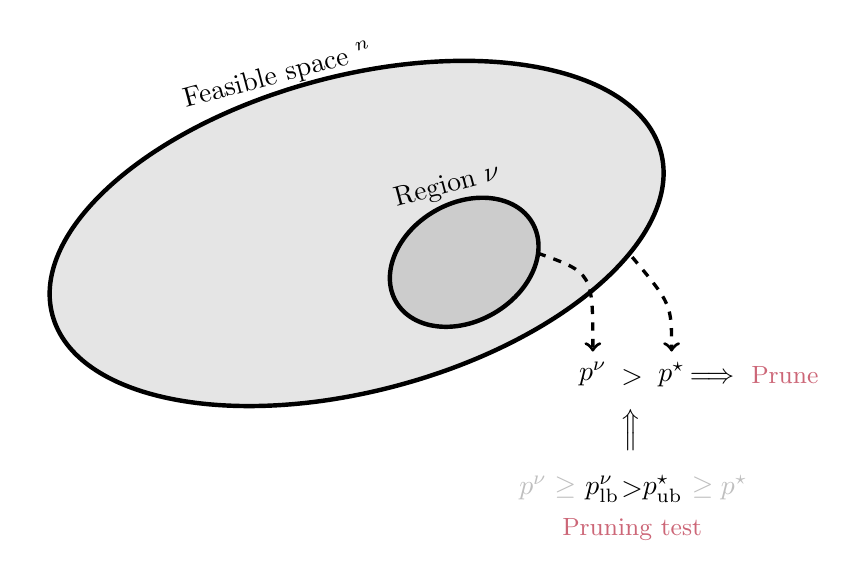
\begin{tikzpicture}
      \draw[ultra thick, fill=gray!20,rotate=15] (0,0) ellipse (4cm and 2cm);
      \node[rotate=15] at (-1,2) {Feasible space $\kR^{\pdim}$};
      \draw[ultra thick, fill=gray!40,rotate=30] (1,-1) ellipse (1cm and 0.75cm);
      \node[rotate=15] at (1.15,0.6) {Region $\nodeSymb$};
      %
      \onslide<2->{
        \draw[dashed, very thick, ->] (2.3,-0.25) ..controls(3,-0.5) .. (3,-1.5) node[below] {$\node{\pobj}$};
        \node[below] at (3.5,-1.6) {$>$};
        \draw[dashed, very thick, ->] (3.5,-0.3) ..controls(4,-0.9) .. (4,-1.5) node[below] {$\opt{\pobj}$};
        \node at (5,-1.8) {$\implies$ \textcolor{TolLightRed}{{\small{Prune}}}};
      }
      \onslide<3->{
        \node at (3.5,-2.5) {\rotatebox[origin=c]{90}{$\implies$}};
        \node at (2.7,-3.25) {$\textcolor{gray!50}{\node{\pobj} \geq} \ \node{\pobj}_{\mathrm{lb}}$};
        \node at (3.5,-3.25) {$>$};
        \node at (4.3,-3.25) {$\opt{\pobj}_{\mathrm{ub}} \ \textcolor{gray!50}{\geq \opt{\pobj}}$};
        \node[below] at (3.5,-3.5) {\textcolor{TolLightRed}{{\small{Pruning test}}}};
      }
    \end{tikzpicture}
  \end{center}
\end{frame}

\begin{frame}{Branch-and-Bound Ingredients}
  \textbf{Region:} $\nodeSymb = (\setzero,\setone,\setnone) \equiv$ partition of $\{1,\dots,\pdim\}$ driving sparsity:
  \begin{itemize}
    \item $\pvi{\idxentry} = 0$ for all $\idxentry \in \setzero$
    \item $\pvi{\idxentry} \neq 0$ for all $\idxentry \in \setone$
    \item $\pvi{\idxentry} \in \kR$ for all $\idxentry \in \setnone$
  \end{itemize}
  ~\\
  \onslide<2->{
    \(
    \begin{array}{llll}
      \opt{\pobj} &= \displaystyle\min_{\pv \in \kR^{\pdim}} \ \lfunc(\pv) + \textcolor{TolLightRed}{\reg\norm{\pv}{0} + \pfunc(\pv)}
      \vspace*{0.3cm}
      \\
      \multicolumn{2}{l}{\downarrow\text{constrainted to region \textcolor{TolLightRed}{$\nodeSymb$}}}
      \vspace*{-0.3cm} \\
      \node{\pobj} &= 
        \displaystyle\min_{\pv \in \kR^{\pdim}} \ \lfunc(\pv) + \textcolor{TolLightRed}{\node{\rfunc}(\pv)}
        \onslide<3->{\quad\text{with}\quad
        \node{\separable{\rfunc}{\idxentry}}(\pvi{\idxentry}) = 
        \begin{cases}
          \icvx(\pvi{\idxentry} = 0) &\text{if } \idxentry \in \setzero \\
          \separable{\pfunc}{\idxentry}(\pvi{\idxentry}) + \reg &\text{if } \idxentry \in \setone \\
          \separable{\pfunc}{\idxentry}(\pvi{\idxentry}) + \reg\norm{\pvi{\idxentry}}{0} &\text{if } \idxentry \in \setnone
        \end{cases}
      }
      \vspace*{-0.4cm}
      \\
      \onslide<4->{
        \rotatebox[origin=c]{90}{$\leq$} \\
        \textcolor{TolLightRed}{\node{\pobj}_{\mathrm{lb}}} & = \text{ optimal value of a } \textcolor{TolLightRed}{\text{relaxation}}
      }
    \end{array}
    \)
  }
  ~\\~\\
  \onslide<5->{
    \begin{center}
      \boxed{
        \text{The relaxation needs to be \textcolor{TolLightRed}{valid}, \textcolor{TolLightRed}{tight} and \textcolor{TolLightRed}{tractable}}
      }
    \end{center}
  }
\end{frame}

\section{Convex Relaxations}

\begin{frame}{Convex Relaxations}
  \vspace*{-0.4cm}
  \textbf{Idea: Convexify the objective function}
  \(
    \begin{array}{lllrl}
      \node{\pobj} &= \displaystyle\min_{\pv \in \kR^{\pdim}} \ \lfunc(\pv) + \textcolor{TolLightRed}{\only<1>{\textcolor{black}}{\node{\rfunc}(\pv)}} & 
      \onslide<2->{
        \text{with} & \node{\separable{\rfunc}{\idxentry}}(\pvi{\idxentry}) =& 
        \begin{cases}
          \icvx(\pvi{\idxentry} = 0) &\text{if } \idxentry \in \setzero \\
          \separable{\pfunc}{\idxentry}(\pvi{\idxentry}) + \reg &\text{if } \idxentry \in \setone \\
          \textcolor{TolLightRed}{\only<1>{\textcolor{black}}{\separable{\pfunc}{\idxentry}(\pvi{\idxentry}) + \reg\norm{\pvi{\idxentry}}{0}}} &\text{if } \idxentry \in \setnone
        \end{cases} \\
      }
      \rotatebox[origin=c]{90}{$\leq$} \\
      \node{\pobj}_{\mathrm{cvx}} 
      \onslide<3->{
        &=  \displaystyle\min_{\pv \in \kR^{\pdim}} \ \lfunc(\pv) + \textcolor{mLightGreen}{\node{\rfunc}_{\text{cvx}}}(\pv) & \text{with} & \node{\separable{\rfunc}{\text{cvx},\idxentry}}(\pvi{\idxentry}) =& 
        \begin{cases}
          \icvx(\pvi{\idxentry} = 0) &\text{if } \idxentry \in \setzero \\
          \separable{\pfunc}{\idxentry}(\pvi{\idxentry}) + \reg &\text{if } \idxentry \in \setone \\
          \textcolor{mLightGreen}{\text{bi-conjugate}} &\text{if } \idxentry \in \setnone
        \end{cases} 
      }
    \end{array}
  \)
  \onslide<4->{
    \begin{center}
      \begin{tikzpicture}
        % \begin{scope}[xshift=-4cm]
        %   \node[above] at (0,1.5) {$\separable{\pfunc}{\idxentry}(\pvi{\idxentry}) = \icvx(\abs{\pvi{\idxentry}} \leq 1)$};
        %   \draw[ultra thick,->] (-1.5,0) -- (1.5,0);
        %   \draw[ultra thick,->] (0,-0.2) -- (0,1.5);
        %   \draw[very thick, TolLightRed] (-1.25,1.5) -- (-1.25,0.5) -- (-0.05,0.5);
        %   \draw[very thick, TolLightRed] (0.05,0.5) -- (1.25,0.5) -- (1.25,1.5);
        %   \draw[very thick, mLightGreen] (-1.28,1.5) -- (-1.28,0.5) -- (0,0) -- (1.28,0.5) -- (1.28,1.5);
        %   \fill[TolLightRed] (0,0) circle (0.075);
        %   \draw[TolLightRed,very thick] (0,0.5) circle (0.075);
        % \end{scope}
        \begin{scope}
          % \node[above] at (0,1.5) {$\separable{\pfunc}{\idxentry}(\pvi{\idxentry}) = \pvi{\idxentry}^2$};
          \draw[ultra thick,->] (-1.5,0) -- (1.5,0);
          \draw[ultra thick,->] (0,-0.2) -- (0,1.5);
          \draw[domain=-1.5:-0.05,smooth,variable=\x,TolLightRed,very thick] plot ({\x}, {0.5 + 0.5*\x*\x});
          \draw[domain=0.05:1.5,smooth,variable=\x,TolLightRed,very thick] plot ({\x}, {0.5 + 0.5*\x*\x});
          \draw[domain=-1.5:-1,smooth,variable=\x,mLightGreen,very thick] plot ({\x}, {0.47 + 0.5*\x*\x});
          \draw[very thick,mLightGreen] (-1,0.97) -- (0,0) -- (1,0.97);
          \draw[domain=1:1.5,smooth,variable=\x,mLightGreen,very thick] plot ({\x}, {0.47 + 0.5*\x*\x});
          \fill[TolLightRed] (0,0) circle (0.075);
          \draw[TolLightRed,very thick] (0,0.5) circle (0.075);
        \end{scope}
        % \begin{scope}[xshift=4cm]
        %   \node[above] at (0,1.5) {$\separable{\pfunc}{\idxentry}(\pvi{\idxentry}) = \abs{\pvi{\idxentry}}$};
        %   \draw[ultra thick,->] (-1.5,0) -- (1.5,0);
        %   \draw[ultra thick,->] (0,-0.2) -- (0,1.5);
        %   \draw[domain=-1.5:-0.05,smooth,variable=\x,TolLightRed,very thick] plot ({\x}, {0.5 - 0.5*\x});
        %   \draw[domain=0.05:1.5,smooth,variable=\x,TolLightRed,very thick] plot ({\x}, {0.5 + 0.5*\x});
        %   \draw[domain=-1.5:1.5,smooth,variable=\x,mLightGreen,very thick] plot ({\x}, {0.5*abs(\x)});
        %   \fill[TolLightRed] (0,0) circle (0.075);
        %   \draw[TolLightRed,very thick] (0,0.5) circle (0.075);
        % \end{scope}
      \end{tikzpicture}
      \\
      {
        \small
        Plot: Functions \textcolor{TolLightRed}{$\node{\separable{\rfunc}{\idxentry}}$} and \textcolor{mLightGreen}{$\node{\separable{\rfunc}{\text{cvx},\idxentry}}$} when $\idxentry \in \setnone$ for $\separable{\pfunc}{\idxentry}(\pvi{\idxentry}) = \pvi{\idxentry}^2$.
      }
    \end{center}
  }
  \vspace*{-1.5cm}
\end{frame}

\begin{frame}{Convex Relaxations}
  \begin{center}
    \textbf{Spotlight Result 1} \\
    \boxed{
      \textbf{The bi-conjugate admits a generic closed-form expression.}
    }
    \\~\\
    Let $\separable{\rfunc}{\idxentry}(\pvi{}) = \separable{\pfunc}{\idxentry}(\pvi{}) + \reg\norm{\pvi{}}{0}$, we have
    \begin{equation*}
      \biconj{\separable{\rfunc}{\idxentry}}(\pvi{}) = 
      \begin{cases}
        \textcolor{mLightGreen}{\separable{\pertslope}{\idxentry}}\abs{\pvi{}} &\text{if } \abs{\pvi{}} \leq \textcolor{mLightGreen}{\separable{\pertlimit}{\idxentry}} \\
        \separable{\pfunc}{\idxentry}(\pvi{}) + \reg &\text{otherwise}
      \end{cases}
    \end{equation*}
    where $(\textcolor{mLightGreen}{\separable{\pertslope}{\idxentry}},\textcolor{mLightGreen}{\separable{\pertlimit}{\idxentry}})$ are some ``easy-to-compute'' quantities.
  \end{center}

  \onslide<2->{
    \begin{center}
      $\downarrow$
    \end{center}
    \begin{center}
      \textbf{Efficient solution methods for the convex relaxation}\\
      \small{Proximal gradient}\\
      \small{Coordinate descent}\\
      \small{Splitting methods}\\
      ...
    \end{center}
  }
\end{frame}

\section{Dual Relaxations}

\begin{frame}{Dual Relaxations}
  \textbf{Idea: Dualize the problem}
  \hspace*{-0.7cm}
  \(
    \begin{array}{lllrl}
      \node{\pobj} &= \displaystyle\min_{\pv \in \kR^{\pdim}} \ \lfunc(\pv) + \node{\rfunc}(\pv) 
      \onslide<4->{
        & \hspace*{-0.2cm} \text{with}\hspace*{-0.2cm}  & \node{\separable{\rfunc}{\idxentry}}(\pvi{\idxentry}) =& \hspace*{-0.2cm} 
        \begin{cases}
          \icvx(\pvi{\idxentry} = 0) &\text{if } \idxentry \in \setzero \\
          \separable{\pfunc}{\idxentry}(\pvi{\idxentry}) + \reg &\text{if } \idxentry \in \setone \\
          \textcolor{TolLightRed}{\separable{\pfunc}{\idxentry}(\pvi{\idxentry}) + \reg\norm{\pvi{\idxentry}}{0}} &\text{if } \idxentry \in \setnone
        \end{cases} \\
      }
      \rotatebox[origin=c]{90}{$\leq$} \\
      \node{\pobj}_{\mathrm{dual}} 
      \onslide<2->{
        &= \displaystyle\max_{\pv \in \kR^{\pdim}} \ -\textcolor{mLightBlue}{\conj{\lfunc}}(-\pv) - \textcolor{mLightBlue}{\conj{(\node{\rfunc})}}(\pv)
      } 
      \onslide<4->{
        & \hspace*{-0.2cm}  \text{with}\hspace*{-0.2cm}  & \conj{(\node{\rfunc})}_{\idxentry}(\pvi{\idxentry}) =& \hspace*{-0.2cm} 
        \begin{cases}
          0 &\text{if } \idxentry \in \setzero \\
          \conj{\separable{\pfunc}{\idxentry}}(\pvi{\idxentry}) - \reg &\text{if } \idxentry \in \setone \\
          \textcolor{mLightBlue}{\text{conjugate}} &\text{if } \idxentry \in \setnone
        \end{cases} 
      }
    \end{array}
  \)
  \onslide<3->{
    \vspace*{-0.5cm}
    \begin{center}
      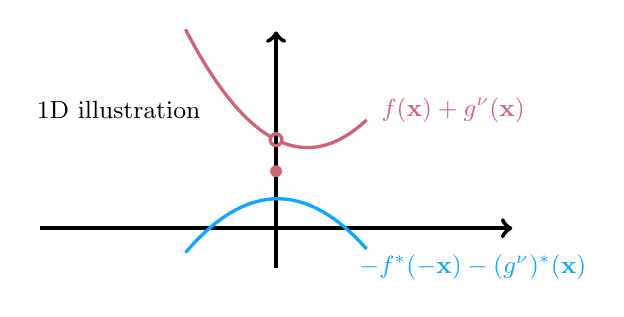
\begin{tikzpicture}
        \draw[ultra thick,->] (-3,0) -- (3,0);
        \draw[ultra thick,->] (0,-0.5) -- (0,2.5);

        \node at (-2,1.5) {\small{1D illustration}};

        \def\aval{1.0}
        \def\yval{0.5}
        \def\lval{0.5}
        \def\bval{0.25}
        \def\ushift{0.52}
        \def\yshift{0.625}

        % Objective
        \draw[TolLightRed,domain=-1.15:-0.075,smooth,variable=\x,very thick] plot (
          {\x},
          {
            0.5 + 0.5 * (\aval * \x - \yval)^2 + \lval + 0.5 * \bval * abs(\x)^2
          }
        );
        \draw[TolLightRed,domain=0.075:1.15,smooth,variable=\x,very thick] plot (
          {\x},
          {
            0.5 + 0.5 * (\aval * \x - \yval)^2 + \lval + 0.5 * \bval * abs(\x)^2
          }
        );
        \draw[TolLightRed,very thick] (0,1.125) circle (0.075);
        \node at (2.25,1.5) {\small\textcolor{TolLightRed}{$\lfunc(\pv) + \node{\rfunc}(\pv)$}};

        % Dual relaxation
        \draw[mLightBlue,domain=-1.15:1.15,smooth,variable=\u,very thick] plot (
          {\u},
          { 0.25 + 
            -0.5 * abs(\u - \ushift)^2 - \yval * (\u - \ushift) - max(0.5 * \bval * \aval * (\u - \ushift)^2 - \lval,0)
          }
        );
        \node at (2.5,-0.5) {\small\textcolor{mLightBlue}{$-\conj{\lfunc}(-\pv) - \conj{(\node{\rfunc})}(\pv)$}};

        % Zero
        \fill[TolLightRed,very thick] (0,0.725) circle (0.075);
      \end{tikzpicture}
    \end{center}
    \vspace*{-1.5cm}
  }
\end{frame}

\begin{frame}{Dual Relaxations}
  \begin{center}
    \textbf{Spotlight Result 2} \\
    \boxed{
      \textbf{The conjugate admits a generic closed-form expression.}
    } 
    \\~\\
    Let $\separable{\rfunc}{\idxentry}(\pvi{}) = \separable{\pfunc}{\idxentry}(\pvi{}) + \reg\norm{\pvi{}}{0}$, we have
    \begin{equation*}
      \conj{\separable{\rfunc}{\idxentry}}(\pvi{}) = 
      \begin{cases}
        0 &\text{if } \abs{\pvi{}} \leq \textcolor{mLightBlue}{\separable{\pertslope}{\idxentry}} \\
        \conj{\separable{\pfunc}{\idxentry}}(\pvi{}) - \reg &\text{otherwise}
      \end{cases}
    \end{equation*}
    where $\textcolor{mLightBlue}{\separable{\pertslope}{\idxentry}}$ is (still) an ``easy-to-compute'' quantity.
  \end{center}

  \onslide<2->{
    \begin{center}
      $\downarrow$
    \end{center}
    \begin{center}
      \textbf{Efficient solution methods for the dual relaxation}\\
      \small{Proximal gradient}\\
      \small{Coordinate descent}\\
      \small{Splitting methods}\\
      ...
    \end{center}
  }
\end{frame}

\begin{frame}{Dual Relaxations}
  \begin{center}
    \textbf{Spotlight Result 3} \\
    \boxed{
      \textbf{\textcolor{mLightGreen}{Convex} relaxations are stronger than \textcolor{mLightBlue}{dual} relaxations.}
    }
  \end{center}

  \begin{center}
    \begin{tikzpicture}
      \draw[ultra thick,->] (-3,0) -- (3,0);
      \draw[ultra thick,->] (0,-1) -- (0,2.5);

      \def\aval{1.0}
      \def\yval{0.5}
      \def\lval{0.5}
      \def\bval{0.25}
      \def\ushift{0.52}
      \def\yshift{0.625}

      % Objective
      \draw[TolLightRed,domain=-1.4:-0.075,smooth,variable=\x,very thick] plot (
        {\x},
        {
          0.5 + 0.5 * (\aval * \x - \yval)^2 + \lval + 0.5 * \bval * abs(\x)^2
        }
      );
      \draw[TolLightRed,domain=0.075:1.4,smooth,variable=\x,very thick] plot (
        {\x},
        {
          0.5 + 0.5 * (\aval * \x - \yval)^2 + \lval + 0.5 * \bval * abs(\x)^2
        }
      );
      \draw[TolLightRed,very thick] (0,1.125) circle (0.075);

      % Convex relaxation
      \draw[mLightGreen,domain=-1.4:1.4,smooth,variable=\x,very thick] plot (
        {\x},
        {
          0.5 + 0.5 * (\aval * \x - \yval)^2 + (
            (abs(\x) < sqrt(2 * \lval / \bval)) * abs(\x / sqrt(2 * \lval / \bval)) + 
            (abs(\x) >= sqrt(2 * \lval / \bval)) * 0.5 * (1 + abs(\x / sqrt(2 * \lval / \bval))^2)
          )
        }
      );

      % Dual relaxation
      \draw[mLightBlue,domain=-1.3:1.3,smooth,variable=\u,very thick] plot (
        {\u},
        {
          -0.5 * abs(\u - \ushift)^2 - \yval * (\u - \ushift) - max(0.5 * \bval * \aval * (\u - \ushift)^2 - \lval,0)
        }
      );

      \node at (-2,1) {\small{1D illustration}};
      \node at (2.25,1.9) {\small\textcolor{TolLightRed}{$\lfunc(\pv) + \node{\rfunc}(\pv)$}};
      \node at (2.25,1.2) {\small\textcolor{mLightGreen}{$\lfunc(\pv) + \node{\rfunc}_{\mathrm{cvx}}(\pv)$}};
      \node at (2.5,-0.9) {\small\textcolor{mLightBlue}{$-\conj{\lfunc}(-\pv) - \conj{(\node{\rfunc})}(\pv)$}};

      \fill[very thick,TolLightRed] (0,0.625) circle (0.075);
    \end{tikzpicture}
  \end{center}

  \vspace*{-0.5cm}

  \onslide<2->{
    But...
    \begin{itemize}
      \item Evaluating the \textcolor{mLightBlue}{dual objective} always gives a valid lower-bound
      \item No need to solve the dual relaxation to optimality
      \item Simple dual link between regions: \textbf{simultaneous pruning}
    \end{itemize}
  }
\end{frame}

\section{Can we do better?}

\begin{frame}{Can we do better?}
  ~\\
  \begin{columns}[T]
    \begin{column}{0.5\textwidth}
      \(
      \begin{array}{lllll}
        \textcolor{TolLightRed}{\node{\pobj}} &= \displaystyle\min_{\pv \in \kR^{\pdim}} \ \lfunc(\pv) + \node{\rfunc}(\pv)
        ~\\
        \rotatebox[origin=c]{90}{$\leq$}
        \onslide<3->{
          ~\\
          \textcolor{mLightBrown}{\node{\pobj}_{\mathrm{ncvx}}} &= \displaystyle\min_{\pv \in \kR^{\pdim}} \ \lfunc(\pv) + \node{\rfunc}_{\mathrm{ncvx}}(\pv)
          ~\\
          \rotatebox[origin=c]{90}{$\leq$}
        }
        ~\\
        \textcolor{mLightGreen}{\node{\pobj}_{\mathrm{cvx}}} &=  \displaystyle\min_{\pv \in \kR^{\pdim}} \ \lfunc(\pv) + \node{\rfunc}_{\text{cvx}}(\pv) \\
        \rotatebox[origin=c]{90}{$\leq$}
        ~\\
        \textcolor{mLightBlue}{\node{\pobj}_{\mathrm{dual}}} &=  \displaystyle\max_{\pv \in \kR^{\ddim}} \ -\conj{\lfunc}(-\pv) - \conj{(\node{\rfunc})}(\pv)
      \end{array}
    \)
    \end{column}
    \hfill
    \begin{column}{0.45\textwidth}
      \begin{tikzpicture}
        \begin{scope}
          \draw[ultra thick,->] (-2,0) -- (2,0);
          \draw[ultra thick,->] (0,-1) -- (0,2.5);
    
          \def\aval{1.0}
          \def\yval{0.5}
          \def\lval{0.5}
          \def\bval{0.25}
          \def\ushift{0.52}
          \def\yshift{0.625}
    
          % Objective
          \draw[TolLightRed,domain=-1.4:-0.075,smooth,variable=\x,very thick] plot (
            {\x},
            {
              0.25 + 0.5 * (\aval * \x - \yval)^2 + \lval + 0.5 * \bval * abs(\x)^2
            }
          );
          \draw[TolLightRed,domain=0.075:1.4,smooth,variable=\x,very thick] plot (
            {\x},
            {
              0.25 + 0.5 * (\aval * \x - \yval)^2 + \lval + 0.5 * \bval * abs(\x)^2
            }
          );
          \draw[TolLightRed,very thick] (0,0.875) circle (0.075);
    
          % Convex relaxation
          \draw[mLightGreen,domain=-1.4:1.4,smooth,variable=\x,very thick] plot (
            {\x},
            {
              0.25 + 0.5 * (\aval * \x - \yval)^2 + (
                (abs(\x) < sqrt(2 * \lval / \bval)) * abs(\x / sqrt(2 * \lval / \bval)) + 
                (abs(\x) >= sqrt(2 * \lval / \bval)) * 0.5 * (1 + abs(\x / sqrt(2 * \lval / \bval))^2)
              )
            }
          );
    
          % Dual relaxation
          \draw[mLightBlue,domain=-1.4:1.4,smooth,variable=\u,very thick] plot (
            {\u},
            {
              -0.5 * abs(\u - \ushift)^2 - \yval * (\u - \ushift) - max(0.5 * \bval * \aval * (\u - \ushift)^2 - \lval,0)
            }
          );
    
          % Stronger relaxation
          \onslide<2->{
            \draw[mLightBrown,domain=-1.4:1.4,smooth,variable=\x,very thick] plot (
              {\x},
              {
                0.25 + 0.5 * (\aval * \x - \yval)^2 + (
                  (abs(\x) < sqrt(2 * \lval * (\aval^2 + \bval)) / (\aval^2 + \bval)) * (sqrt(2 * \lval * (\aval^2 + \bval)) * abs(\x) - 0.5 * abs(\x)^2 * (\aval^2 + \bval)) +
                  (abs(\x) >= sqrt(2 * \lval * (\aval^2 + \bval)) / (\aval^2 + \bval)) * \lval
                ) + 0.5 * \bval * abs(\x)^2
              }
            );
          }
    
          \fill[very thick,TolLightRed] (0,0.4) circle (0.06);
        \end{scope}
      \end{tikzpicture}
    \end{column}
  \end{columns}

  ~\\
  \onslide<4->{
    \begin{center}
      \textbf{Reminder}~\\\vspace*{0.1cm}
      \boxed{
        \text{The relaxation needs to be valid, tight and tractable}
      }
    \end{center}
  }
  \onslide<5->{
    \begin{enumerate}
      \item Validity $\quad \, \, $: $\node{\rfunc}_{\mathrm{ncvx}} \leq \node{\rfunc}$
      \item Tightness$\ \ \, $: $\node{\rfunc}_{\mathrm{ncvx}} \geq \node{\rfunc}_{\mathrm{cvx}}$
      \item Tractability: $\lfunc + \node{\rfunc}_{\mathrm{ncvx}}$ is convex
    \end{enumerate}
  }
\end{frame}

\begin{frame}{Can we do better?}
  \begin{columns}[T]
    \begin{column}{0.6\textwidth}
      \textbf{Least-squares loss and $\boldsymbol{\ell}_2$-norm penalty}
      ~\\~\\
      \(
        \begin{array}{lllll}
          \opt{\pobj} &= \displaystyle\min_{\pv \in \kR^{\pdim}} \ \tfrac{1}{2}\norm{\obs-\dic\pv}{2}^2 + \textcolor{TolLightRed}{\reg \norm{\pv}{0} + \tfrac{\regtwo}{2}\norm{\pv}{2}^2}
          ~\\
          \rotatebox[origin=c]{90}{$\leq$}
          \onslide<2->{
            ~\\
            \opt{\pobj}_{\mathrm{ncvx}} &=  \displaystyle\min_{\pv \in \kR^{\pdim}} \ \tfrac{1}{2}\norm{\obs-\dic\pv}{2}^2 + \textcolor{mLightBrown}{\textsc{Mcp}_{\mcpone,\mcptwo}(\pv) + \tfrac{\regtwo}{2}\norm{\pv}{2}^2}
            ~\\
            \rotatebox[origin=c]{90}{$\leq$}
          }
          ~\\
          \opt{\pobj}_{\mathrm{cvx}} &=  \displaystyle\min_{\pv \in \kR^{\pdim}} \ \tfrac{1}{2}\norm{\obs-\dic\pv}{2}^2 + \textcolor{mLightGreen}{\textsc{Berhu}_{\reg,\regtwo}(\pv)}
        \end{array}
      \)
    \end{column}
    \hfill
    \begin{column}{0.3\textwidth}
      \vspace*{1cm}
      \begin{tikzpicture}
        \def\tauval{1.224744871391589}
        \def\muval{1.224744871391589}
        \def\mcptwoval{2}
        \def\mcponeval{1.7320508075688772}

        \draw[ultra thick,->] (-1.5,0) -- (1.5,0);
        \draw[ultra thick,->] (0,-0.2) -- (0,1.5);

        \draw[domain=-1.5:-0.05,smooth,variable=\x,TolLightRed,very thick] plot ({\x}, {0.75 + 0.5*\x*\x});
        \draw[domain=0.05:1.5,smooth,variable=\x,TolLightRed,very thick] plot ({\x}, {0.75 + 0.5*\x*\x});

        \draw[domain=-1.5:-\muval,smooth,variable=\x,mLightGreen,very thick] plot ({\x}, {0.7 + 0.5*\x*\x});
        \draw[very thick,mLightGreen] (-\muval,1.45) -- (0,0) -- (\muval,1.45);
        \draw[domain=\muval:1.5,smooth,variable=\x,mLightGreen,very thick] plot ({\x}, {0.7 + 0.5*\x*\x});

        \onslide<2->{
          \draw[domain=-1.5:1.5,smooth,variable=\x,mLightBrown,very thick] plot (
            {\x},
            {
              (
                (abs(\x) < sqrt(2 * 0.75 * (\mcponeval^2 + \mcptwoval)) / (\mcponeval^2 + \mcptwoval)) * 
                  (
                    sqrt(2 * 0.75 * (\mcponeval^2 + \mcptwoval)) * abs(\x) - 0.5 * abs(\x)^2 * (\mcponeval^2 + \mcptwoval)
                  ) 
                +
                (abs(\x) >= sqrt(2 * 0.75 * (\mcponeval^2 + \mcptwoval)) / (\mcponeval^2 + \mcptwoval)) * 0.75
              ) + 0.5 * abs(\x)^2 - 0.025
            }
          );
        }

        \fill[TolLightRed] (0,0) circle (0.075);
        \draw[TolLightRed,very thick] (0,0.75) circle (0.075);
      \end{tikzpicture}
    \end{column}
  \end{columns}
  ~\\~\\~\\
  \onslide<3->{
    Sufficient conditions:
    \begin{itemize}
      \item $\textcolor{mLightBrown}{\mcpone} = \sqrt{2\reg\textcolor{mLightBrown}{\mcptwo}} \qquad\qquad\qquad \ \, \rightarrow\quad$ validity and tightness \ding{52}
      \item $\transp{\dic}\dic + \regtwo\Id - \diag(\textcolor{mLightBrown}{\mcptwo}) \succeq \0 \quad\rightarrow\quad$ tractability  \ding{52}
    \end{itemize}
  }
\end{frame}

\begin{frame}

  \begin{center}
    \Large{\textbf{Takeways}}
  \end{center}
  \begin{itemize}
    \item Generalizing BnB $\equiv$ Generic \textcolor{TolLightRed}{relaxation} in a given region
    \begin{itemize}
      \item Generic \textcolor{mLightGreen}{convex} relaxation
      \item Generic \textcolor{mLightBlue}{dual} relaxation
      \item Both having their own advantages
    \end{itemize}
    \item Can we do better?
    \begin{itemize}
      \item \textcolor{mLightBrown}{Non-convex} relaxation of the penalty
      \item Tune parameters to ensure validity, tightness and tractability
      \item Case with least-squares loss and $\ell_2$-norm penalty
      \item We'll see next if it works in practice!
    \end{itemize}
  \end{itemize}
\end{frame}

\begin{frame}[standout]

  \vspace*{2cm}
  Question time!
  \vspace*{1.5cm}

  \begin{center}
    \normalsize
    \textbf{We are building a benchmark for sparse problems with} \\
    
\includegraphics[width=0.3\textwidth]{img/logo_benchopt_white.png} \\
    \textbf{We are looking for contributors, datasets, solvers, ...} \\
    \textbf{Feel free to join!}
  \end{center}
\end{frame}

\end{document}
